\documentclass[a4paper, 10pt, danish, final]{article}
\usepackage{bonde}

\def\mytitle{Dataanalyse 2010}
\def\mysubtitle{Aflevering af ugeopgave 4}
\def\myauthor{Ulrik Bonde}
\def\mymail{\mailto{bonde@diku.dk}}
\def\mydate{\today}
\def\repository{\url{http://github.com/bonde/dataanalyse}}

\title{\mytitle}
\subtitle{\mysubtitle}

\author{\myauthor{} - \mymail}
\date{\mydate}

\hypersetup{
colorlinks,%
citecolor=black,%
filecolor=black,%
linkcolor=black,%
urlcolor=black,%
bookmarksopen=false,
pdftitle={\mytitle{} - \mysubtitle},
pdfauthor={\myauthor}
}

\begin{document}
\maketitle

\subsection*{Spørgsmål 1}
Den totale population vi betragter er alle mænd og kvinder. Da det ikke
er muligt at undersøge hele populationen bruges en stikprøve. Der ønskes
at undersøgt hvorvidt kvinder snakker mere end mænd. I de følgende
overvejelser antages det at kvinder faktisk taler mere end mænd.

Vi skal nu overveje hvorvidt vores stikprøve er tilfældig og
repræsentativ. Ifølge opgaveteksten består fem af de seks stikprøver af
universitetsstuderende, men ifølge \citep{mehl2007women} er alle
deltagere i forsøget universitetsstuderende. Endvidere er alle deltagere
i stikprøve 2 til 6 fundet gennem psykologikurser. Endeligt spænder
alderen af de undersøgte mellem 17 -- 29 år. Da alle mænd og kvinder
ikke studerer psykologi på universitetet og ikke er mellem 17 -- 29 år,
mener jeg ikke man kan sige at stikprøven er tilfældig.

Der nævnes i \citep{mehl2007women} at stikprøvernes sammensætning
muligvis kan have påvirket resultatet. Dog kan vi sige, at \emph{hvis}
kvinder virkelig snakker mere end mænd, så må vi også forvente at
resultater fra vores stikprøve afspejler dette (på trods af indtægt,
interesser og alder). Vi ønsker kun at se på forholdet mellem antallet
af ord der udtales af mænd og kvinder. Med mindre det vides, at et
givent køn snakker mere hvis de er universitetsstuderende, kan den givne
data godt anses for at være repræsentativ med henblik på undersøgelsens
formål.

Som sidebemærkning til det ovenstående, er det dog interessant at kigge
på kønsfordelingen i de enkelte prøver. Uden at virke alt for
fordomsfuld, kunne man godt forestille at der blev snakket mere eller
mindre på kurser med en skæv kønsfordeling. Det supplerende materiale
til \citep{mehl2007women} viser dog at kønsfordelingen er nogenlunde
lige. Endelig bliver antallet af ord optaget med et apparat som virker
døgnet rundt, dvs. der optages også selvom personen ikke befinder sig på
studiet.

Vi ser nu på om stikprøven er \emph{independent and identically
distributed}. Vi antager at de enkelte forsøg er uafhængige. Dvs. at den
samme person ikke deltager i flere forsøg, f.eks. på i forsøg nr. 1 og
2. Det supplerende materiale til \citep{mehl2007women} nævner ikke noget
om uafhængighed, men vi må antage at dette holder. Stikprøverne er taget
over flere år (1998 --- 2004) hvilket taler for stikprøvernes
uafhængighed. Stikprøverne skal endvidere have den samme
sandsynlighedsfordeling. Man kan godt overbevise sig selv om at dette
også holder, hvilket der delvist er argumenteret for ovenfor. Man kan
også kigge på histogrammet over alle prøverne --- som illustreret i
figur \ref{dists_iid} --- og se at de følger samme mønster.

\begin{figure}[h]
    \centering
    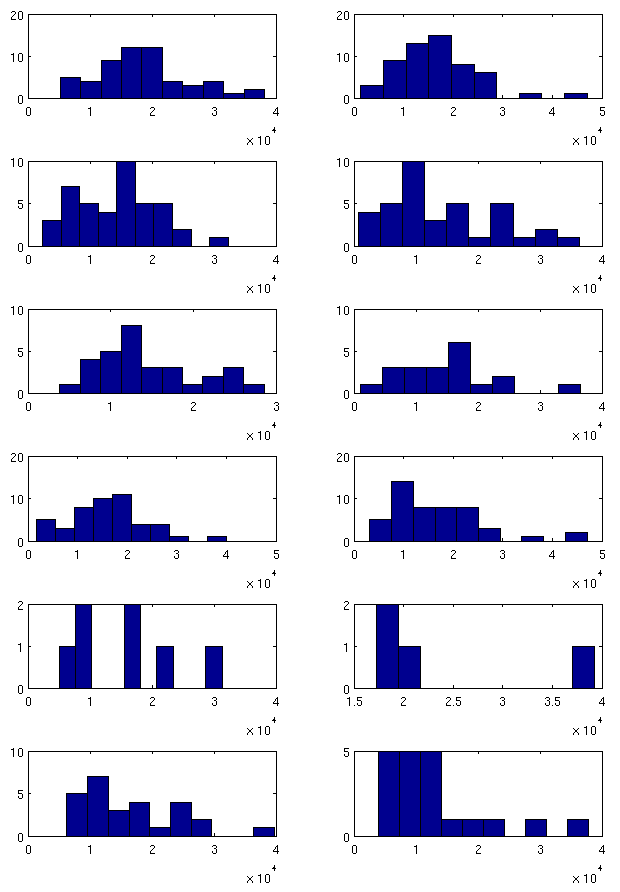
\includegraphics[width=0.95\textwidth]{images/dists_iid}
    \caption{Histogrammer for stikprøve 1 -- 6. Første række viser prøve
    nr. 1 med kvinder til venstre og mænd til højre. Anden række er for
    prøve nr. 2 etc.. Det ses at histogrammet for alle prøver nogenlunde
    følger samme fordeling.}
    \label{dists_iid}
\end{figure}

Udvælgelsen kunne være foretaget ved stratifikation. Man kunne f.eks.
godt forestille sig at man også havde kørt forsøget på en gruppe af
ikke-universitetsstuderende. Forholdet mellem de to grupper skulle da
være lig forholdet i hele populationen, dvs. verden. Dette ville også
kunne afsløre \emph{hvis} mandlige psykologistuderende af en eller grund
skulle snakke mere end andre mænd. Jeg tror dog ikke det er tilfældet og
udvælgelse ved stratifikation ville blot gøre forsøget dyrere. Der
findes mange andre måder at inddele populationen på, f.eks.
nationalitet, indkomst og/eller hvorvidt man tuder når man skærer løg.

\subsection*{Spørgsmål 2}
Det der kunne forhindre at alle M-data og alle F-data sammen kunne være
hvis de enkelte stikprøver ikke var uafhængige og/eller havde vidt
forskellige fordelinger, dvs. hvis de ikke var \emph{'iid'}. Der er
allerede argumenteret for dette ovenfor og i figur \ref{dists_iid}.

Endvidere findes en række andre teknikker --- hentet fra EDA
\citep[kap. 5]{1199778} --- som kan bruges til at afgøre hvorvidt alle
M- og F-data har samme fordelingsfunktion. Af disse kan nævnes
\emph{q-q plot}, hvor vi har samme fordelingsfunktion hvis punkterne
ligger på en ret linje, samt varianter af \emph{boxplot} hvor vi får en
mere grafisk repræsentation af kvartiler og fordelingerne. Sidstnævnte
er en mere kompakt udgave af figur \ref{dists_iid}, men kræver lidt
MATLAB-vold når vi ikke har samme antal målinger i stikprøverne.

\subsection*{Spørgsmål 3}
Ved brug af de vedlagte MATLAB-programmer er størrelserne middelværdi
($\mu$), varians ($\sigma^2$), $\gamma_1$ og $\gamma_2$ fundet. Disse er
opstillet i tabel \ref{emp}.

Vi har i tabellen også lagt alle M og F-data sammen. Det ses at
Brizendines påstand ikke holder. Vi ser på middelværdierne, hvor kvinder
taler ca. 16215 ord og mænd omkring 15669. Disse tal --- og forholdet
mellem dem --- stemmer på ingen måde overens med det oprindelige udsagn.

\begin{table}
    \centering
    \begin{tabular}{|c|c|c|c|c|c|}
        \hline
        & \textbf{Sample no.} & $\mu$ & $\sigma^2$ & $\gamma_1$ & $\gamma_2$\\
        \hline
        \multirow{7}{*}{\textbf{Female}}
        & 1 & 18443.250000 & 55646054.190909 & 0.524084 & 3.028171 \\
        & 2 & 14296.690476 & 41486057.243322 & 0.371198 & 2.865104 \\
        & 3 & 14704.064516 & 38630580.462366 & 0.634373 & 2.605101 \\
        & 4 & 16177.085106 & 56542570.949121 & 0.432775 & 3.856698 \\
        & 5 & 15761.285714 & 80739735.238095 & 0.574349 & 2.312762 \\
        & 6 & 16496.111111 & 62636860.256410 & 0.958396 & 3.726311 \\
        \hline
        & All & 16215.028571 & 53307887.348462 & 0.606659 & 3.416344 \\
        \hline
        \hline
        \multirow{7}{*}{\textbf{Male}}
        & 1 & 16576.142857 & 61960195.106494 & 1.231019 & 5.989515 \\
        & 2 & 14060.378378 & 82174848.797297 & 0.633930 & 2.539597 \\
        & 3 & 15021.850000 & 61840397.923684 & 0.688443 & 4.159915 \\
        & 4 & 16568.857143 & 82961957.791667 & 1.243791 & 5.020865 \\
        & 5 & 24050.750000 & 104260620.250000 & 1.083780 & 2.277796 \\
        & 6 & 12866.700000 & 69596842.115789 & 1.639661 & 5.364589 \\
        \hline
        & All & 15668.526882 & 74520654.866841 & 1.036650 & 4.539524 \\
        \hline
    \end{tabular}
    \caption{Empiriske størrelser}
    \label{emp}
\end{table}

\subsection*{Spørgsmål 4 og 5}
Vi vil nu prøve at finde frem til hvilken teoretisk fordeling vi kan
bruge til at beskrive vores data. Til dette visualiseres data som
histogrammer vist i figur \ref{hists}.

Fordelingen, som vi ser fra histogrammerne med $n = 18$ (fig.
\ref{hist_f_18} og \ref{hist_m_18}), kan godt ligne en normalfordeling.
Vi ved dog fra spørgsmål 3, hvor vi har fundet $\gamma_2$-værdierne, at
fordelingerne er ``skarpere'' end en normalfordeling. I histogrammerne
ser fordelingen også ud til at være lidt skæv, hvilket igen er indikeret
af positive værdier af $\gamma_1$. Derfor kunne der godt kunne være tale
om en gamma- eller poisson-fordeling.

\begin{figure}[!h]
    \centering
    \subfloat[Kvinder. $n = 9$.]{\label{hist_f_9}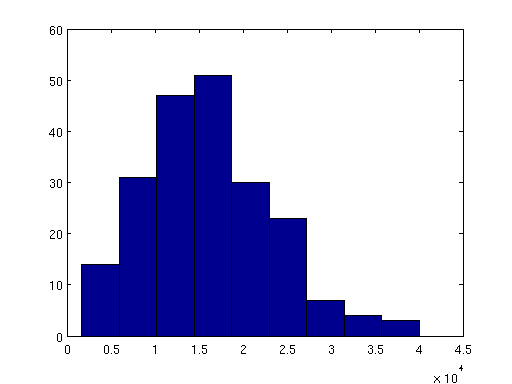
\includegraphics[angle=0,width=0.45\textwidth]{images/hist_f_9}\hspace{1em}}
    \subfloat[Mænd. $n = 9$.]{\label{hist_m_9}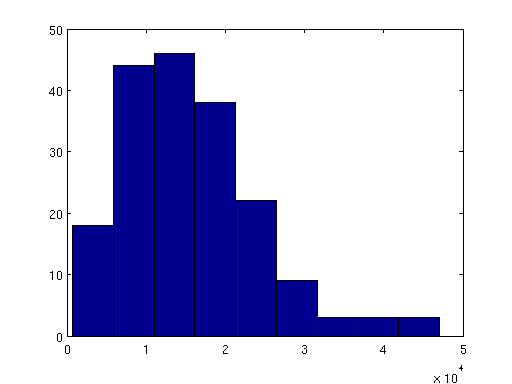
\includegraphics[angle=0,width=0.45\textwidth]{images/hist_m_9}}\\
    \subfloat[Kvinder. $n =
    18$.]{\label{hist_f_18}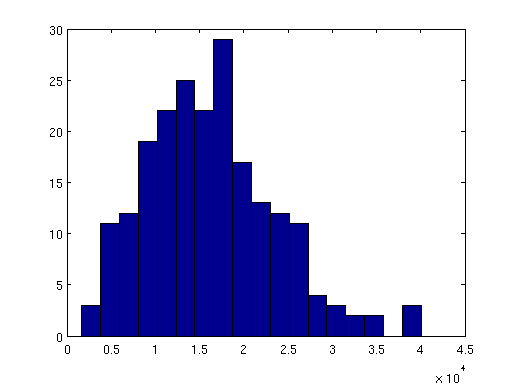
\includegraphics[angle=0,width=0.45\textwidth]{images/hist_f_18}\hspace{1em}}
    \subfloat[Mænd. $n =
    18$.]{\label{hist_m_18}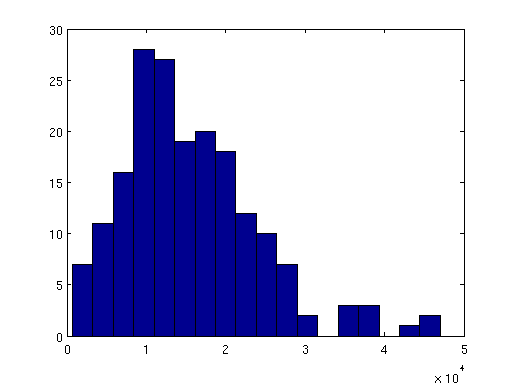
\includegraphics[angle=0,width=0.45\textwidth]{images/hist_m_18}}\\
    \subfloat[Kvinder. $n =
    30$.]{\label{hist_f_30}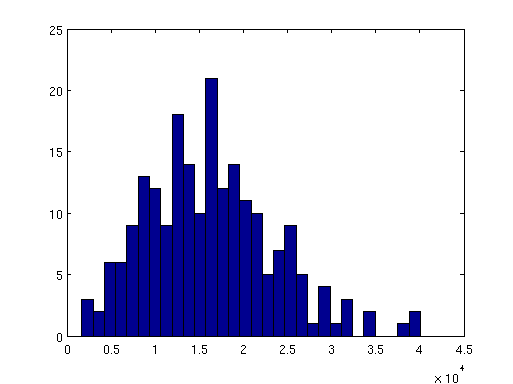
\includegraphics[angle=0,width=0.45\textwidth]{images/hist_f_30}\hspace{1em}}
    \subfloat[Mænd. $n =
    30$.]{\label{hist_m_30}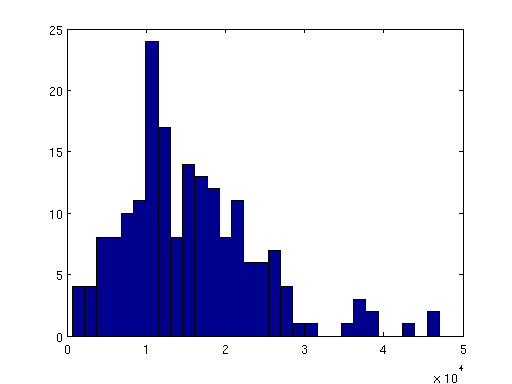
\includegraphics[angle=0,width=0.45\textwidth]{images/hist_m_30}}
    \caption[]{Histogrammer af hhv. alle F og M-data med forskellige
    antal grupperinger ($n$). Når vi bruger for mange grupperinger
    bliver fordelingsfunktionen sværere at genkende. Omvendt kan for få
    grupperinger også antyde en forkert fordeling. Det bedste resultat
    ses omkring 18.
    }
    \label{hists}
\end{figure}

\clearpage

%%%%%%%%%%%%%%%%%%%%%%%%%%%%%%%%%%%%%%%%%%%%%%%%%%%%%%%%%%%%%%%%%%%%
% Formal stuff

\bibliographystyle{abbrvnat}
\bibliography{bibliography}
%\addcontentsline{toc}{chapter}{Litteratur}

\appendix
\lstset{language=Matlab, basicstyle=\scriptsize,
    showstringspaces=false, numbers=left, stepnumber=1,
    numberstyle=\tiny, frame=none}
\section{Kildekode}
Kildekoden er tilgængelig i mit git-repository på \repository{}. Bemærk
at prefikset \texttt{DA} står for ``DataAnalyse'' og blot er til for at
undgå eventuelle sammenstød med indbyggede funktioner i MATLAB.

\subsection{week4.m}
\lstinputlisting{../src/week4.m}

\subsection{PrintStat.m}
\lstinputlisting{../src/PrintStat.m}

\subsection{DASkewness.m}
\lstinputlisting{../src/DASkewness.m}

\subsection{DAKurtosis.m}
\lstinputlisting{../src/DAKurtosis.m}

\end{document}

% vim: set tw=72 spell spelllang=da:
